\begin{frame}{Frame Title}

    \begin{block}{title\{\textit{text}\}, date\{\textit{text}\}, author\{\textit{text}\} y maketitle\{\}}
    Especificamos \textit{título}, \textit{fecha} y \textit{autores}*, y luego en el cuerpo del documento, creamos el la portada antes que nada.
    \end{block}

    \pause
    
    \begin{columns}
        \column{0.5\textwidth}
            \hspace{1.5cm}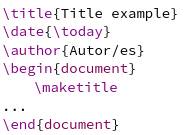
\includegraphics[width=0.5\textwidth]{images/make_title.png}
        \pause
        \column{0.5\textwidth}
            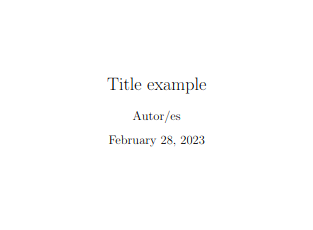
\includegraphics[width=\textwidth]{images/make_title_res.png}
    \end{columns}

    \pause

    \centering
    \textit{O podemos crear la portada mano...}

\end{frame}